\section{Resultados}
Os resultados alcançados demonstram a capacidade do motor gráfico desenvolvido 
em representar com sucesso primitivas geométricas complexas e configurar cenários 
dinâmicos como o sistema solar. As primitivas geométricas, especificamente o Cone 
e a Esfera, foram implementadas com precisão, permitindo uma visualização detalhada 
e realista destas formas tridimensionais. A implementação do sistema solar, tanto em
uma orientação horizontal quanto em uma configuração mais tradicional, reflete a 
flexibilidade e a robustez do motor gráfico. Essas implementações são cruciais para 
a visualização de cenários astronômicos e a compreensão da disposição espacial dos 
corpos celestes.

\break
\noindent
Os resultados a que se chegou podem, então ser observados nas Figuras
\ref{fig:boneconeve}, \ref{fig:sissolarhor} e \ref{fig:sissolar}.

\subsection{Cone e Esfera}

\begin{center}
    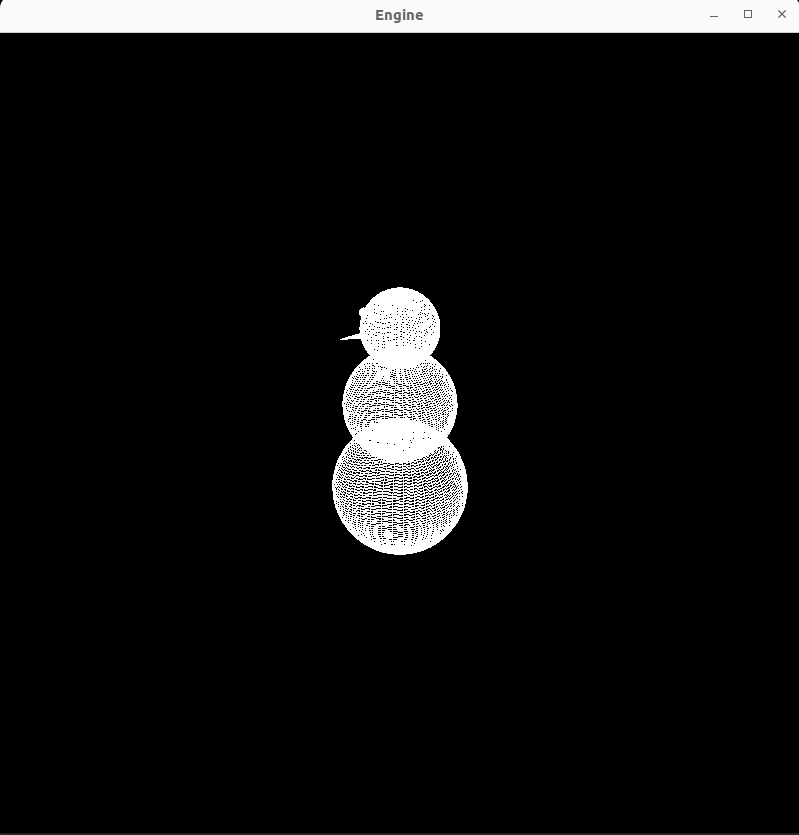
\includegraphics[width=0.8\textwidth]{../imgs/boneconeve.png}
    \captionof{figure}{Cone e Esfera implementados}
    \label{fig:boneconeve}
\end{center}

\subsection{Sistema Solar Horizontal}

\begin{center}
    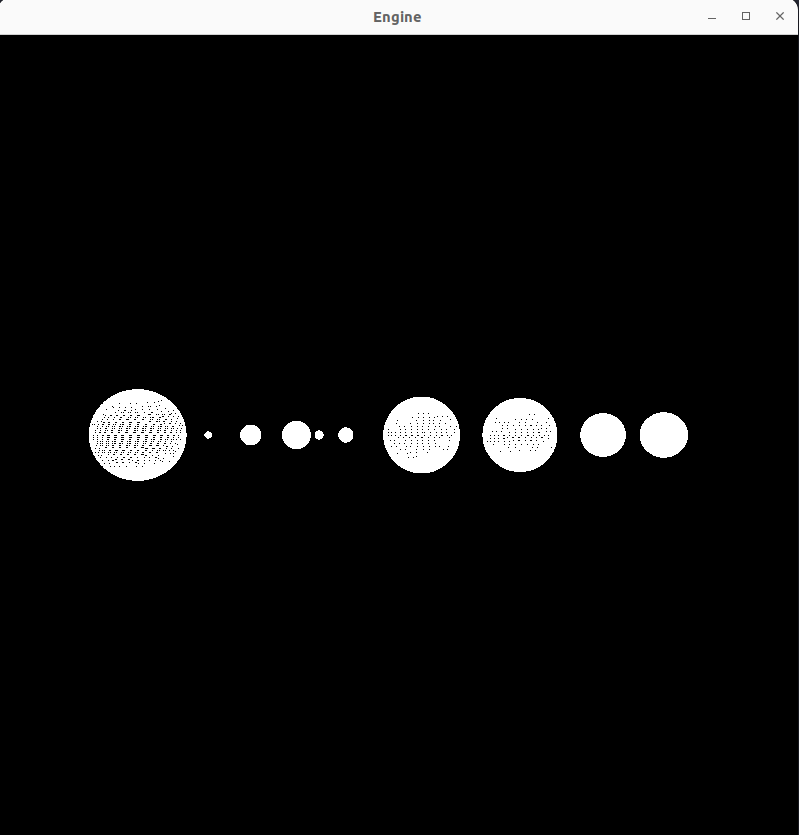
\includegraphics[width=0.8\textwidth]{imgs/sissolarhor.png}
    \captionof{figure}{Sistema Solar Horizontal implementado}
    \label{fig:sissolarhor}
\end{center}

\subsection{Sistema Solar}

\begin{center}
    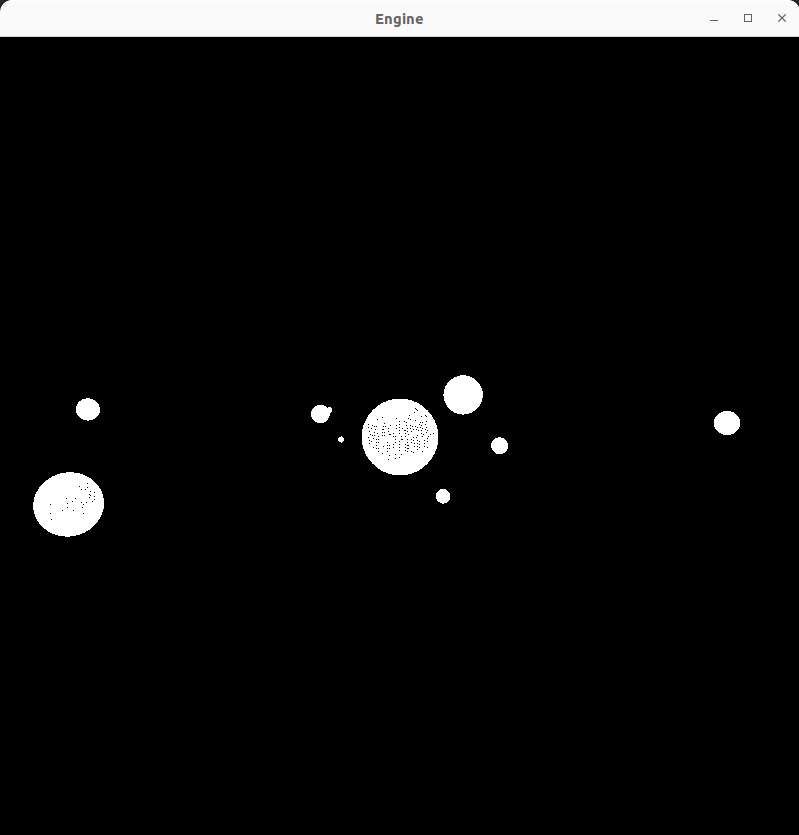
\includegraphics[width=0.8\textwidth]{imgs/sissolar.png}
    \captionof{figure}{Sistema Solar implementado}
    \label{fig:sissolar}
\end{center}